\chapter{Explaining complex codon usage patterns with selection for translational efficiency, mutation bias, and genetic drift}\label{ch:treff}
This chapter is a lightly revised version of a paper by the same name submitted in Proc. Natl. Acad. Sci. and co-authored with Michael A. Gilchrist.\\

\clearpage
\pagebreak

%\begin{abstract} 
\section*{\centering Abstract}
The genetic code is redundant with most amino acids using multiple codons.
In many organisms, codon usage is biased towards particular codons.
Understanding the adaptive and non-adaptive forces driving the evolution of codon usage bias (CUB) has been an area of intense focus and debate in the fields of molecular and evolutionary biology.
However, their relative importance in shaping genomic patterns of CUB remains unsolved.
Using a nested model of protein translation and population genetics, we show that observed gene level variation of CUB in \emph{S. cerevisiae} can be explained almost entirely by selection for efficient ribosomal usage, genetic drift and biased mutation.
The correlation between observed codon counts within individual genes and our model predictions is 0.96.
Although a variety of factors shape patterns of CUB at the level of individual sites within genes, our results suggest that selection for efficient ribosome usage is a central force in shaping codon usage at the genomic scale.
In addition, our model allows direct estimation of codon-specific mutation rates and elongation times and can be readily applied to any organism with high throughput expression datasets.
More generally, we have developed a natural framework for integrating models of molecular processes to population genetics models to quantitatively estimate parameters underlying fundamental biological processes such as protein translation.
%\end{abstract}

\clearpage
\pagebreak

\section{Introduction}
For many organisms the preferential use of certain codons, commonly referred to as codon usage bias (CUB), is strongly correlated with corresponding tRNA abundances and expression levels \citep{Ikemura81,DongEtAl96}.
Explanations for these correlations abound; the most favored ones include selection against translational errors \citep{Akashi94,DrummondAndWilke09,Gilchrist07}, selection for translational efficiency \citep{Bulmer91,AkashiAndEyreWalker98,ColemanEtAl08},  effects on protein folding \citep{KimchiSarfatyEtAl07}, and stability of mRNA secondary structures \citep{KudlaEtAl09,TullerEtAl10b}.
Since different combinations of these factors could lead to very similar patterns of codon usage, their relative importance in shaping evolution of CUB is unknown \citep{AravaEtAl05,KudlaEtAl09,ShahAndGilchrist10b}.
We believe that this uncertainty over their relative importance is, in large part, due to lack of mechanistic models of processes hypothesized to give rise to these patterns (for exceptions see \citep{Bulmer91,GilchristAndWagner06,ShahAndGilchrist10b}).
While most theories of codon usage predict that the degree of bias in codon usage should increase with gene expression \citep{Ikemura81,DrummondAndWilke09,GilchristEtAl09}, they lack any specific quantitative predictions about the rate and nature of these changes.
This is because most commonly used indices of CUB, such as  $F_\text{\emph{op}}$ \citep{Ikemura81}, \emph{CAI} \citep{SharpAndLi86}, and \emph{CBI} \citep{BennetzenAndHall82}, are both heuristic and aggregate measures of CUB and fail to explicitly define the factors responsible for the evolution of CUB  (for exceptions see \citep{dosReisEtAl04,GilchristEtAl09}).
In contrast, we show that a mechanistic model of protein translation that explicitly includes the effects of biased mutation, genetic drift, and selection for efficient ribosome usage can explain the genome wide codon usage patterns in \emph{S. cerevisiae}.
Although, ours is not the first attempt at using mechanistic models to explain CUB in a population genetics context \citep{Bulmer91,Gilchrist07}, it is unique in its ability to estimate codon-specific parameters and quantitatively predict how codon frequencies change with gene expression.
We find that our model can explain $\sim$92\% of the observed variation in CUB across the \emph{Saccharomyces cerevisiae} genome.

\section{Model}
Protein synthesis is the most energetically expensive process within a cell \citep{Wagner05}.
During the log-phase of growth in \emph{S. cerevisiae}, about 60\% of transcriptional machinery is devoted to making about 2000 ribosomes every minute \citep{Warner99}. 
Since ribosomes are large complexes with finite lifespan and are expensive to manufacture, one would expect strong selection for their efficient use during protein translation \citep{Kurland87,Bulmer91,LovmarAndEhrenberg06,HershbergAndPetrov08}.
%Despite its importance, the majority of work on codon usage biases has focused on the effect of translation errors (Fig. 1).
Here we explicitly define selection for efficient use of ribosomes as selection for translational efficiency \citep{Bulmer91,LovmarAndEhrenberg06}.
Since codons that have longer elongation times tie up ribosomes on the mRNA leading to an inefficient usage, these codons should be selected against. 
Thus, in the absence of other factors, selection for translation efficiency should favor coding sequences that use codons with shorter elongation times and the strength of this selection should increase with gene expression \citep{Bulmer91,AkashiAndEyreWalker98,Akashi03,HershbergAndPetrov08}.
If selection for translational efficiency is a major force driving the evolution of CUB in \emph{S. cerevisiae}, then we should be able to predict the CUB of a gene based on the differences in elongation times of synonymous codons, mutational bias, and its expression level.

We model the cost of protein production explicitly in terms of ATP usage as it is common currency for energy consumption within a cell \citep{Alberts08}.
Based on the work in \citep{Gilchrist07,GilchristEtAl09}, we begin our model by first noting that in the absence of translation errors, the expected cost for production of a single protein is simply
\begin{align}
\eta(\vec{x})&=C\sum_{i=1}^{61}x_it_i,
\end{align}
where $x_i$ is the number of codons of type $i$ among the 61 sense codons used within a given coding sequence $\vec{x} = \{x_1, x_2, \ldots x_{61}\}$, $t_i$ is the expected elongation time for codon $i$, and $C$ is a scaling factor that represents the overhead cost of ribosome usage in ATP/sec.
Codons that have shorter elongation times will lead to lower costs $\eta$, and hence, are expected to be selected over their coding synonyms.
Based on the work in \citep{Gilchrist07,GilchristEtAl09} we assume an exponential fitness function $w(\vec{x}|\phi)\propto e^{-q\phi\eta(\vec{x})}$, where $q$ is the scaling constant (sec/ATP) determining the relationship between the rate of ATP usage and fitness $w$ and $\phi$ is a measure of gene expression, specifically protein production rate (proteins/sec).
It is important to note the distinction between the protein production rate and the translation rate of a ribosome across an mRNA.
This lack of distinction has been the source of confusion over the role of gene expression in shaping patterns of codon usage in the past \citep{Bulmer91,PlotkinAndKudla11}.

In addition, although protein production rate of a gene changes during a single cell's lifetime, the $\phi$ value used here is the target time-averaged rate at which the protein will be produced.
%In other words, $\phi$ represents the expected number of functional proteins to be produced over the lifetime of a cell.
In this scenario, a change from an optimal codon to a suboptimal codon does not affect $\phi$ but instead affects the cost of meeting the target $\phi$.
Using the cost of producing a protein $\eta$ as the phenotype, we calculate the probability of observing a particular coding sequence given its expression level, $P(\vec{x}|\phi)$. 
$P(\vec{x}|\phi)$ is defined for each coding sequence in the synonymous codon genotype space $S_c$ for a given protein.
Under the Fisher-Wright process \citep{Wright69,Gavrilets04B,SellaAndHirsh05} this probability is,
\begin{align}
P\left(\vec{x}|\phi\right)&\propto w\left(\vec{x}|\phi\right)^{N_e}\prod_{i=1}^{61}\mu_i^{x_i}%}{\sum_{y\in S_c}w\left(\vec{y}|\phi\right)^{N_e}\prod_{i=1}^{61}\mu_i^{y_i}}
\end{align}
where $N_e$ is the effective population size and $\mu_i$ is the sum of mutation rates to codon $i$ from its synonymous codons \citep{SellaAndHirsh05}.
Simply put, $P(\vec{x}|\phi)$, the probability of observing a particular synonymous codon genotype for a given protein is a combined function of mutation bias $\prod_{i=1}^{61}\mu_i^{x_i}$, natural selection for translational efficiency $w$, and genetic drift $N_e$.
Given an expression level $\phi$, the probability of observing a set of codons for one amino acid is independent of the probability of observing a set of codons for another amino acid (Section \ref{text:c4_1}).
This independence allows us to calculate the expected frequencies of codons within an amino acid independent of codon compositions of other amino acids.
The resulting expected frequency of codon $i$ of amino acid $aa_k$ that has $n_k$ synonymous codons is given by
\begin{align}
\mathbb{E}[f_i|\phi,aa_k]&=\frac{\mu_ie^{-N_e q C \phi t_i}}{\sum_{j\in n_k}\mu_je^{-N_e q C \phi t_j}}.
\end{align}

Equation 3 describes how the expected frequency of a given codon changes with gene expression $\phi$ at its mutation-selection-drift equilibrium.
In order to compare our model predictions to observed codon usage frequencies, we looked at the 4674 verified nuclear genes that lack internal stops in \emph{S. cerevisiae} \citep{Gilchrist07,ShahAndGilchrist10b}.
Since time-average target protein production rates of genes are not available for any organism, we use estimates of protein production rates during log growth as proxies.
Empirical estimates of protein production rates $\phi$ were obtained from \citep{Gilchrist07}, which combines mRNA abundance \citep{BeyerEtAl04} and ribosome occupancy datasets \citep{AravaEtAl03,MacKayEtAl04,ShahAndGilchrist10b}.
The effective population size was set to $N_e=1.36\times10^7$ based on the effective population size of its closely related species \emph{S. paradoxus} \citep{Wagner05}.
Note that because $N_e$ is scaled by $qC$ in Eqn. 3, any error in our estimate of $N_e$ will only affect our estimates of $qC$ and not the behavior of our predictions.

% Results and Discussion can be combined.
\section{Results}

\subsection{Model Behavior.}
The general behavior of our model is illustrated in Fig. \ref{fig:c4_1}, which shows the simple case of one amino acid with two codons.
It demonstrates how expected frequencies of the codons change with gene expression with respect to \emph{differences} in the elongation times of the codons $\Delta t_{ij}=t_i-t_j$ as well and their relative mutation rates $\mu_i/\mu_j$.
As expected, codon usage in genes with low expression is primarily determined by their relative mutation rates, while codon usage in genes with high expression is determined by the differences in their elongation times.
When both natural selection for translation efficiency and mutation biases favor the same codon, the lines representing expected frequencies of codons (red lines in Fig. 1) do not cross.
However, when the direction of mutation bias is opposite to that of natural selection, the lines representing expected frequencies of codons cross (blue lines in Fig. \ref{fig:c4_1}).

\begin{figure}[H]
        \begin{center}
                %\includegraphics[width=0.9\textwidth]{./Figures/tmp3.pdf}
               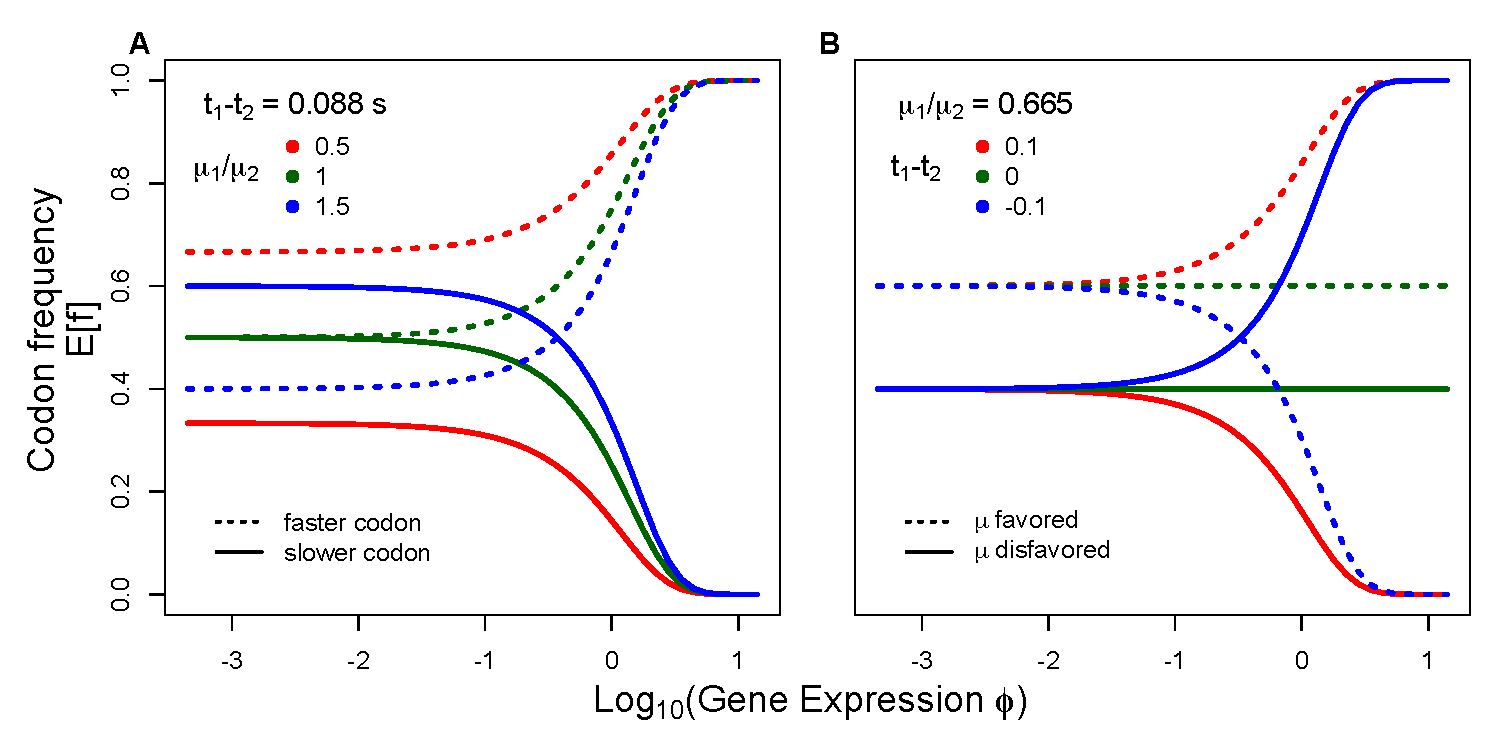
\includegraphics[width=0.9\textwidth]{../Figure/c4Fig_1.pdf}
	\end{center}
	\caption{Effect of varying relative mutation rates ($\mu_i/\mu_j$), elongation times ($\Delta t_{ij}$) and protein production rate ($\phi$) on the expected codon frequencies ($\mathbb{E}[f]$) in a hypothetical two-codon amino acid.}
	%Solid and dashed lines represent the frequencies of the two synonymous codons.
	\textbf{A} Effect of changing $\mu_i/\mu_j$ on $\mathbb{E}[f]$ with $\phi$.
	Solid lines represent the codon with longer elongation time $t_1$ and dotted lines represent the codon with shorter elongation time $t_2$.
	Mutation bias has a greater effect on $\mathbb{E}[f]$ at low $\phi$, while at very high $\phi$, the $\mathbb{E}[f]$ of codons converge to the same values irrespective of $\mu_i/\mu_j$.
	\textbf{B} Effect of changing $t_i-t_j$ on their expected frequencies $\mathbb{E}[f]$ with respect to $\phi$.
	Solid lines represent the codon with a lower relative mutation rate $\mu_1$ and dotted lines represent the codon with a higher mutation rate $\mu_2$.
	Differences in elongation times between the two codons $t_1-t_2$ has little effect on $\mathbb{E}[f]$ at low $\phi$.
	However, at high $\phi$, as $t_1-t_2$ changes, so does the difference in their expected frequencies $\mathbb{E}[f]$. 
	\label{fig:c4_1}
\end{figure}


\subsection{Model Fit to {\it S. cerevisiae} Genome.}
We calculated maximum likelihood estimates for the composite parameter $qC$, codon-specific differences in elongation times $\Delta t_{ij}$, and relative mutation rates $\mu_i/\mu_j$ using 4674 genes of the \emph{S. cerevisiae} genome (see Section \ref{sec:meth}, Table \ref{table:c4_2}, Table \ref{table:c4_3} for more details).

\begin{table}[H]
\caption{Estimates of relative mutation rates $\mu_i/\mu_j$}
\label{table:c4_2}
\centering
                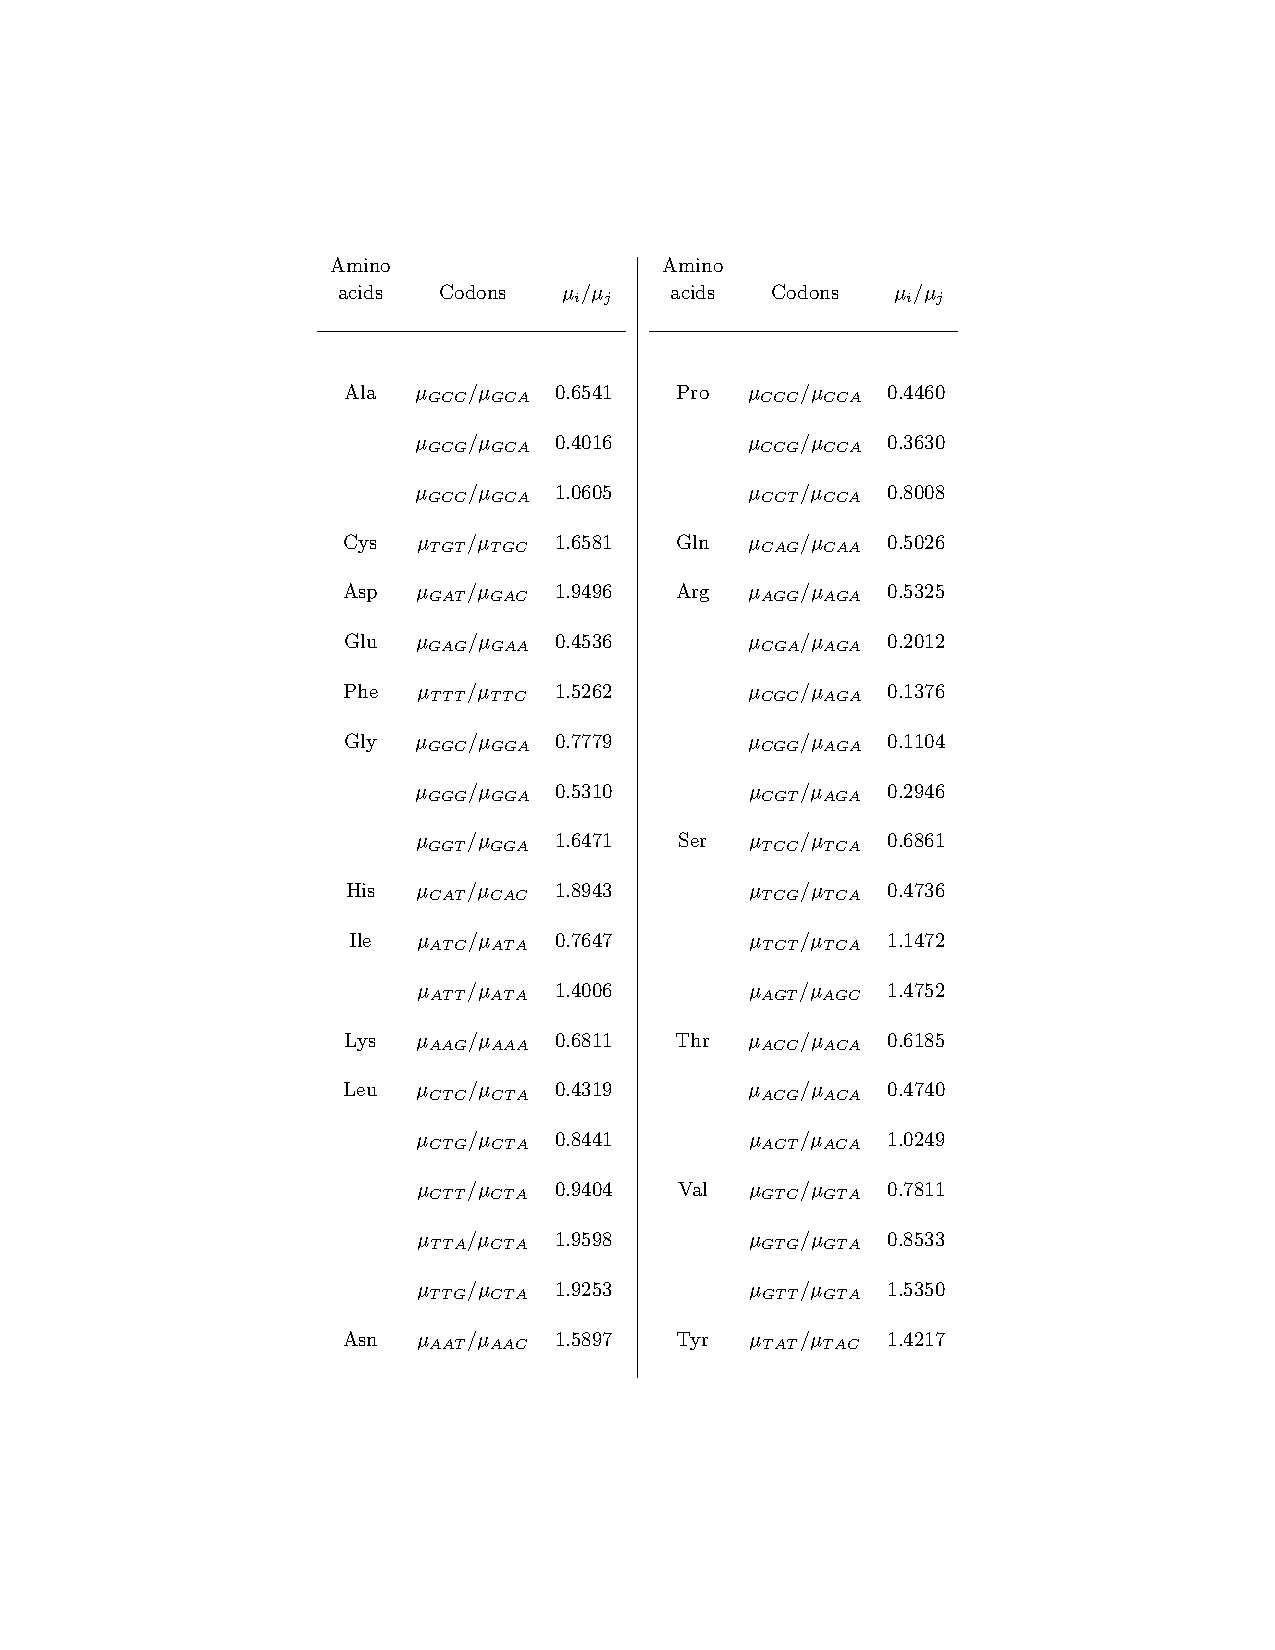
\includegraphics[width=0.76\fullwidth]{../Figure/c4Tab_2.pdf}
\end{table}

\begin{table}
\caption{Estimates of differences in elongation times $\Delta t$ (s)}
\label{table:c4_3}
\centering
                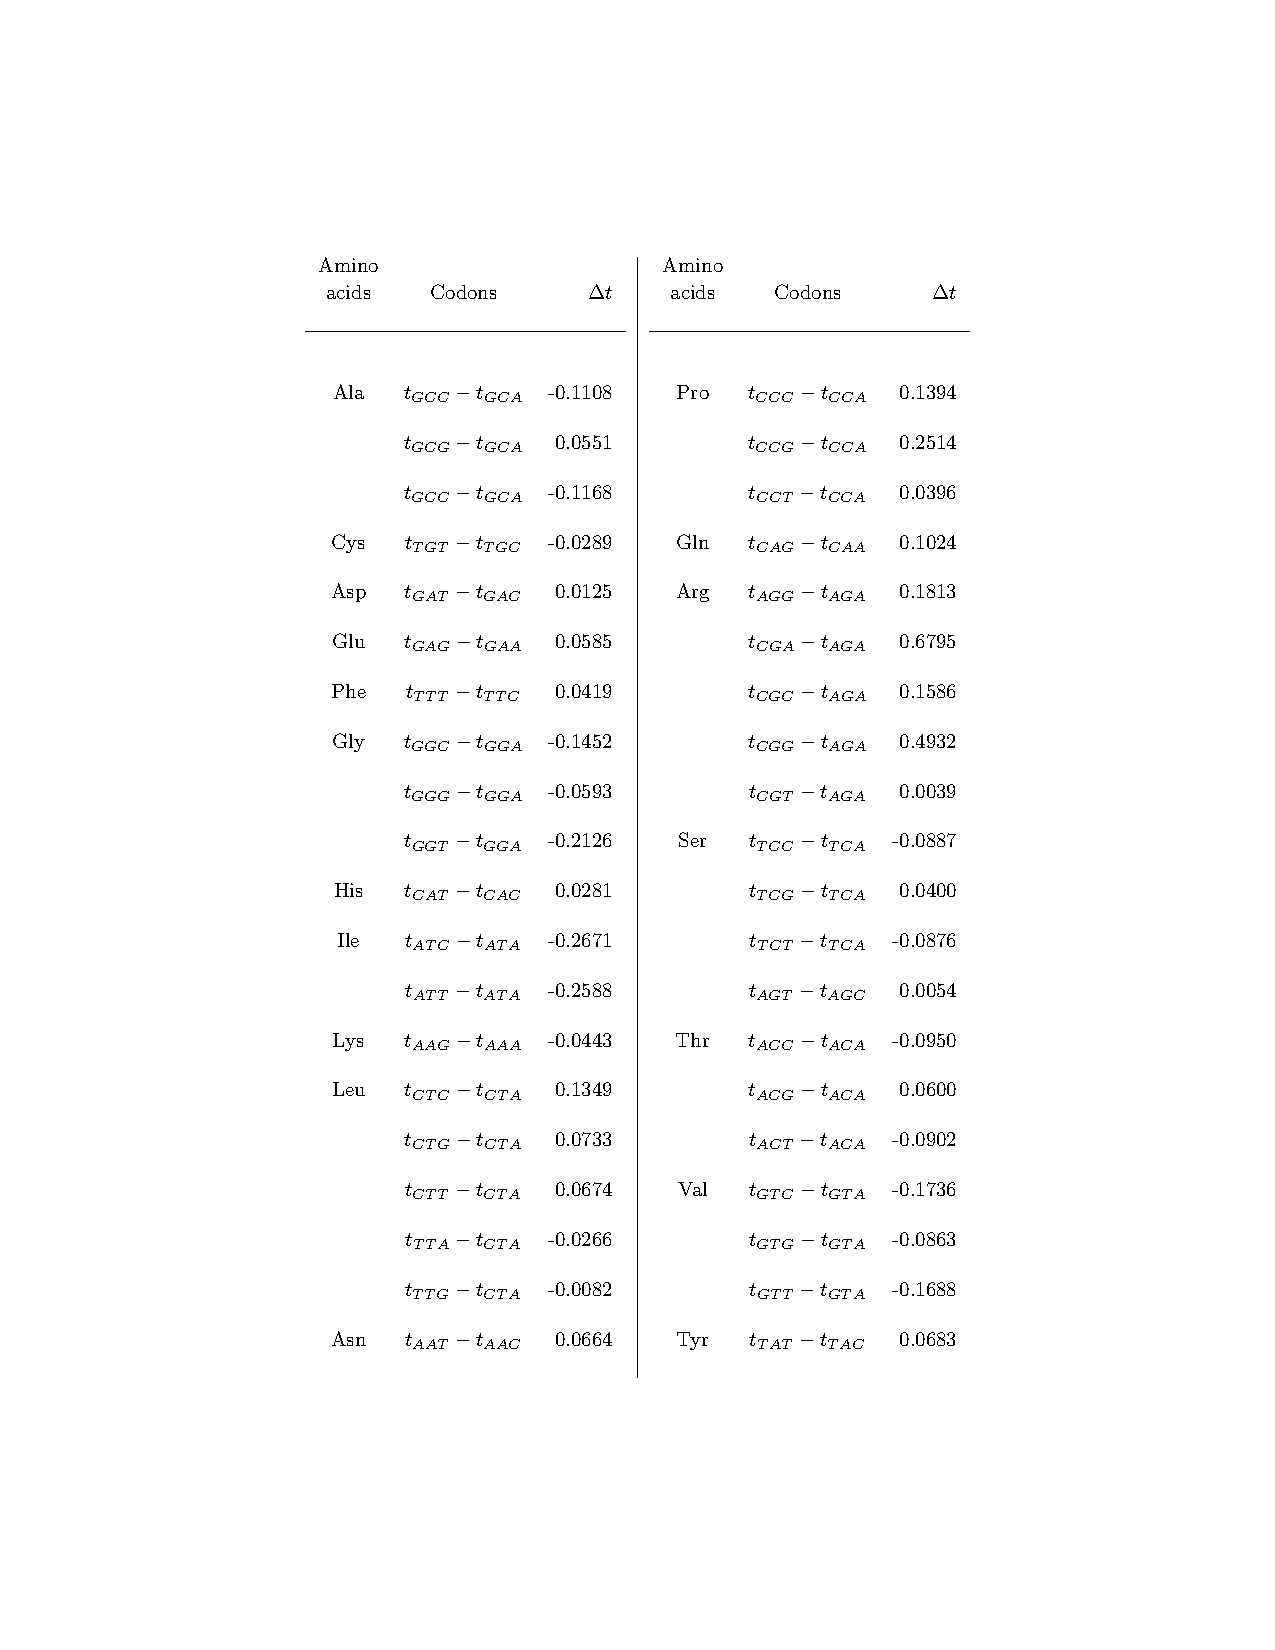
\includegraphics[width=0.76\fullwidth]{../Figure/c4Tab_3.pdf}
\end{table}


Although, our model uses $2(k-1)$ parameters for each amino acid with $k$ codons, we show that it is far from being over-parameterized as it uses genome scale datasets (see Section \ref{text:c4_2}).
%At worst, the ratio of number of data points to parameters for an amino acid was $\sim$400.
The fit of our model predictions with observed data is illustrated in Fig. \ref{fig:c4_2}.
Specifically, Fig. \ref{fig:c4_2} shows how the observed and predicted codon frequencies change with gene expression $\phi$ for all the amino acids that use multiple codons.
Because the set of synonymous codons for Ser occur in blocks of  two and four codons separated by more than a single mutation step, we treat each of the blocks as a separate amino acids, Ser$_2$ and Ser$_4$ respectively.
The fit of our model can be quantified on a per amino acid basis based on the Pearson correlation $\rho_M$ between mean of binned observed codon frequencies and predicted codon frequencies at mean $\phi$ value.  
The $\rho_M$ values ranged from 0.72 to 0.99 with a median value of 0.936.

\begin{figure}[H]
        \begin{center}
                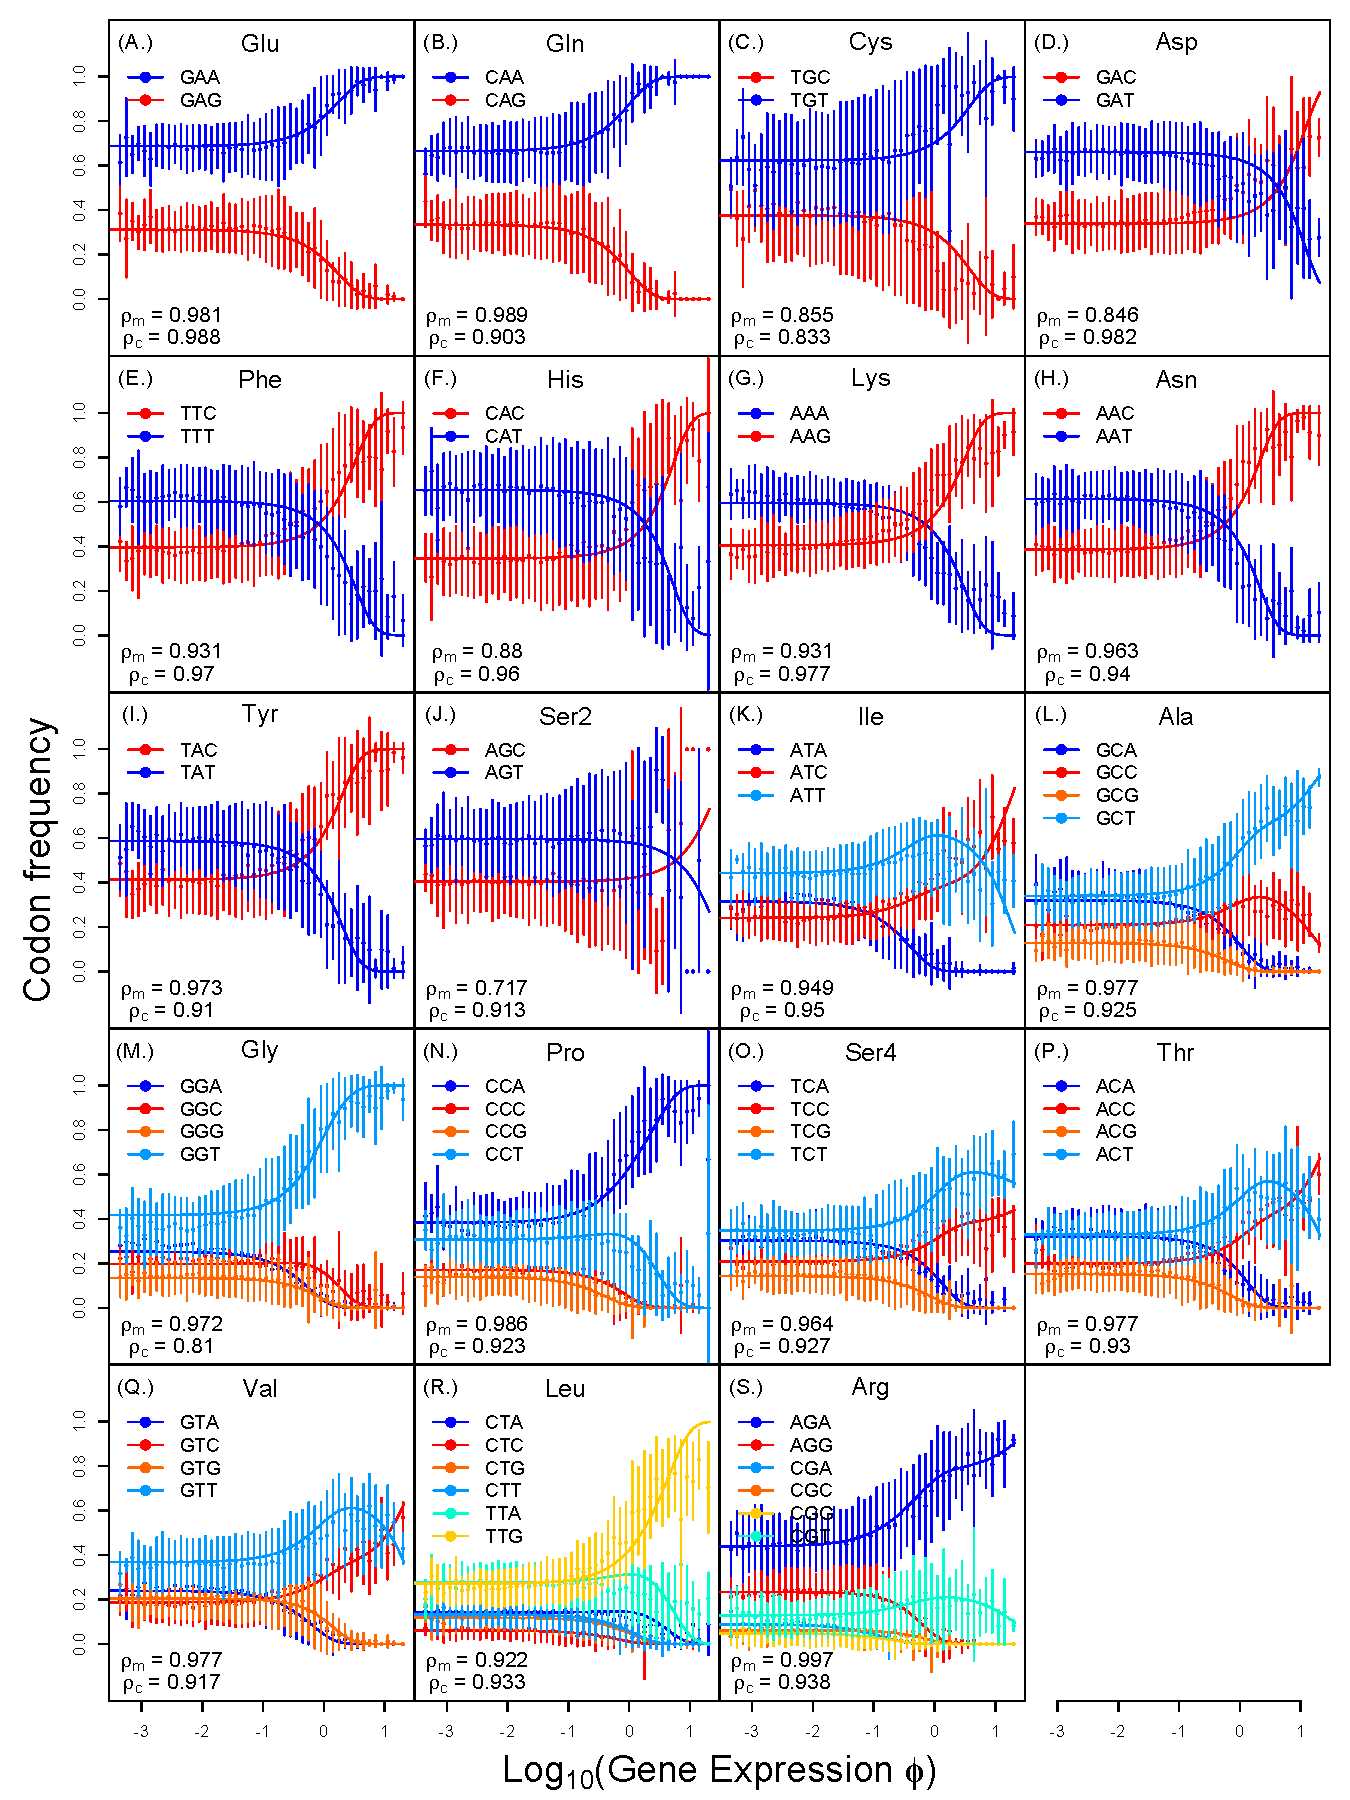
\includegraphics[width=0.75\textwidth]{../Figure/c4Fig_2.pdf}
	\end{center}
	\caption{Observed and predicted changes in codon frequencies with gene expression, specifically protein production rate $\phi$.}
	Each panel corresponds to a specific amino acid where codons ending in A or T are is shown in shades of blue while codons ending in G or C in shades of red.
	Solid dots and vertical bars represent mean $\pm 1$ SD of observed codon frequencies within genes with protein production rates defined by the bin. 
	The expected codon frequencies under our model are represented by solid lines.
	We used $k-1$ codons of an amino acid with $k$ codons in estimating correlation coefficients.
	$\rho_M$ represents the Pearson correlation between the mean of observed codon frequencies within a bin and predicted codon frequencies at mean $\phi$ value. 
	$\rho_c$ represents the Pearson correlation between observed codon counts and predicted codon counts of all genes at their specific $\phi$ value.
%	We combined data from all but one codons of an amino acid to correct for the degrees of freedom in calculating correlation coefficients.
%	Our model also captures the non-monotonic changes in codon frequencies with gene expression observed in every amino acid with $>2$ synonymous codons.
	\label{fig:c4_2}
\end{figure}

Although many indices of adaptation have been proposed to estimate the degree of codon bias within a gene, there exists no method or index that makes predictions on codon counts of individual genes itself.
For instance, if a particular gene has a protein production rate $\phi$, what should the distribution of its codons be given its amino acid sequence?
%In order to directly address this, we compared the observed codon counts within each gene with codon counts predicted under our model using estimates of $\Delta t_{ij}$ and $\mu_i/\mu_j$ (Table \ref{table:c4_4}).
In order to directly address this question we used our estimates of $\Delta t_{ij}$ and $\mu_i/\mu_j$ (Table \ref{table:c4_2}, Table \ref{table:c4_3}) to evaluate on a per-gene basis the expected codon frequencies for each amino acid using Eqn. 3. 
We find that the correlation between observed and predicted codon counts is $\rho_c=0.959$ (Fig. \ref{fig:c4_3}), explaining $\sim92\%$ of observed variation in codon counts.
Even at the level of individual amino acids, the correlation coefficients $\rho_c$ ranged from $0.81-0.99$.
All but two amino acids had $\rho_c>0.9$, indicating that the high correlation was consistent across all amino acids.
In summary, we find that our model does an excellent job of predicting how the observed codon frequencies in \emph{S. cerevisiae} change with gene expression $\phi$.

\begin{figure}[H]
        \begin{center}
                %\includegraphics[width=0.9\textwidth]{./Figures/tmp3.pdf}
                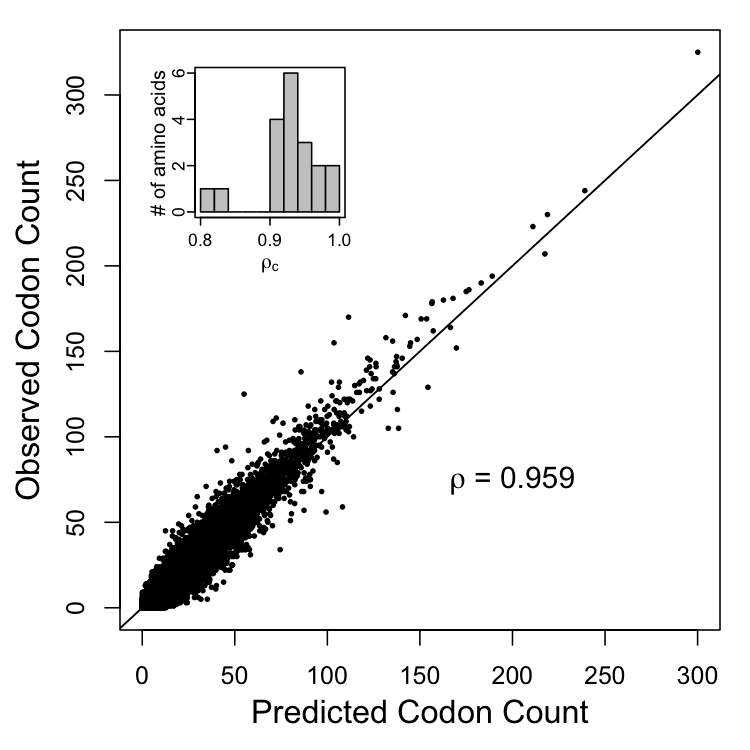
\includegraphics{../Figure/c4Fig_3.pdf}
	\end{center}
	\caption{Correlation between observed codon counts and predicted codon counts of individual genes.}
	We used codon counts of $k-1$ codons of an amino acid with $k$ codons.
	Ignoring Met and Trp (one codon amino acids) and splitting Ser into two blocks of four and two codons, there are 19 unique amino acid sets.
	Hence the number of data points used are $4674\times(59-19)=186,960$.
	We find a very high correlation ($\rho=0.959$, $p$-value $<10^{-15}$) between our model predictions and observed counts.
	Inset shows the distribution of correlation coefficients at the level of individual amino acids, indicating that our high correlation is not biased by specific amino acids and that we have a high correlation across all amino acids.
	\label{fig:c4_3}
\end{figure}

One key insight from this work is that in \emph{S. cerevisiae} for amino acids with more than two codons, the frequencies of preferred codons with similar elongation times $\Delta t_{ij}$ can change in a non-monotonic manner with gene expression $\phi$.
For instance, in the case of Thr, the frequency of codon ACT increases from low to moderate levels of gene expression log($\phi$) but decreases at high gene expression and is replaced by codon ACC.
This non-monotonic behavior is the result of complex interplay between mutation biases and translation selection.
Specifically, although both the codons ACC and ACT have shorter elongation times than their other coding synonyms ACG and ACA, codon ACC has the shortest elongation time.
However, unlike codon ACC, ACT is favored by mutation bias, so its frequency initially increases with gene expression.
We call this phenomenon `mutational inertia', whereby, the frequency of a suboptimal codon transiently increases with gene expression due to mutation bias.
This non-monotonic behavior runs counter to traditional explanations where the frequency of an optimal codon is expected to monotonically increase and that of a suboptimal codon to monotonically decrease with gene expression \citep{SharpAndLi86,DuretAndMouchiroud99}.
We observed these effects of mutational inertia in most of the amino acids with more than two codons.
Although non-monotonic changes in codon frequencies with gene expression have been previously documented \citep{Bulmer88}, the mechanisms responsible for this behavior have not been put forth.
We believe this interesting and complex interplay between mutation biases and selection for efficient translation has been obscured due to an overemphasis on indices in studies of codon usage bias.
Our study illustrates the advantages of model-based approach used here over heuristic approaches.
In addition and as indicated by the crossing of lines representing codon frequencies, 7 out of 10 amino acids with two codons in Fig. \ref{fig:c4_2} (D-J), show mutation biases in a direction opposite to that of natural selection.
In other words, codons with high frequencies in low expression genes are not the same as the ones preferred in high expression genes.
Along with explaining these previously described patterns \citep{SharpAndDevine89,MustoEtAl03,PeixotoEtAl04}, we quantity the changes in codon frequencies with gene expression.

In addition to describing the genome scale patterns of codon usage, our model also allows for estimation of relative mutation rates $\mu_i/\mu_j$ and differences in  elongation times of these codons $\Delta t_{ij}$ on a per amino acid basis directly from the genome sequence and expression datasets.
%We find that using a simple multinomial model for the distribution of codon counts suffices to describe codon usage in genes with low expression and estimation of relative mutation rates (see Methods for details).
Interestingly, we find that estimates of relative mutation rates sometimes differed between amino acids. 
For instance, in the case of two-codon amino acids (Lys, Gln, and Glu) the NNA codons were always favored over NNG codons.
However, the relative mutation rate $\mu_{NNG}/\mu_{NNA}$ ranged from 0.45-0.68 with a mean of 0.546.
These small but significant differences (t test, $p<10^{-9}$ for every pair of amino acids) in the estimation of relative mutation rate may be due, in part, to the fact that our model does not allow for non-synonymous substitutions, some of which may behave in a nearly neutral manner, especially in genes with low $\phi$ values.

We also compared our estimates of $\Delta t_{ij}$ with estimates based on tRNA gene copy numbers as proxy for tRNA abundances and wobble penalties (see Methods).
%To scale the estimates of elongation times of codon, we used inverse of elongation rates based on tRNA gene copy numbers from \citep{GilchristAndWagner06,Gilchrist07}.
We find that these independently obtained estimates of $\Delta t_{ij}$ are highly correlated ($\rho=0.801$) (Fig. \ref{fig:c4_4}). 

\begin{figure}[H]
        \begin{center}
                %\includegraphics[width=0.9\textwidth]{./Figures/tmp3.pdf}
                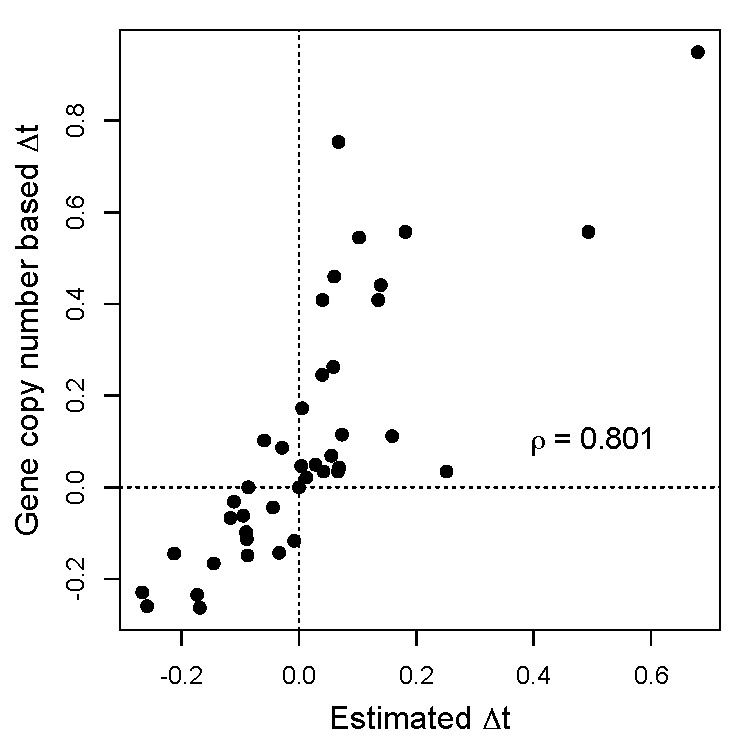
\includegraphics{../Figure/c4Fig_4.pdf}
	\end{center}
	\caption{Correlation between our model based estimates of $\Delta t_{ij}$s with $\Delta t_{ij}$s estimated using tRNA gene copy numbers.}
	We find a strong correlation ($\rho=0.801$, $p$-value $<10^{-9}$) between our model estimates and estimates of $\Delta t_{ij}$ based on tRNA gene copy numbers indicating that our estimates can be related to other biological estimates such as tRNA abundances directly.
	\label{fig:c4_4}
\end{figure}


\subsection{Model Fit vs. Model Predictions.}
In order to demonstrate the predictive value of our model, we randomly partitioned the \emph{S. cerevisiae} genome into two sets of 2337 genes each with no signifiant bias in their distribution of gene expression levels $\phi$ (t test, $p>0.4$).
Parameters estimated using half the genome were found to be highly correlated with our previous estimates based on the entire genome $\rho>0.99$ for both $\Delta t_{ij}$ and $\mu_i/\mu_j$ (Fig. \ref{fig:c4_5}).

\begin{figure}[H]
        \begin{center}
                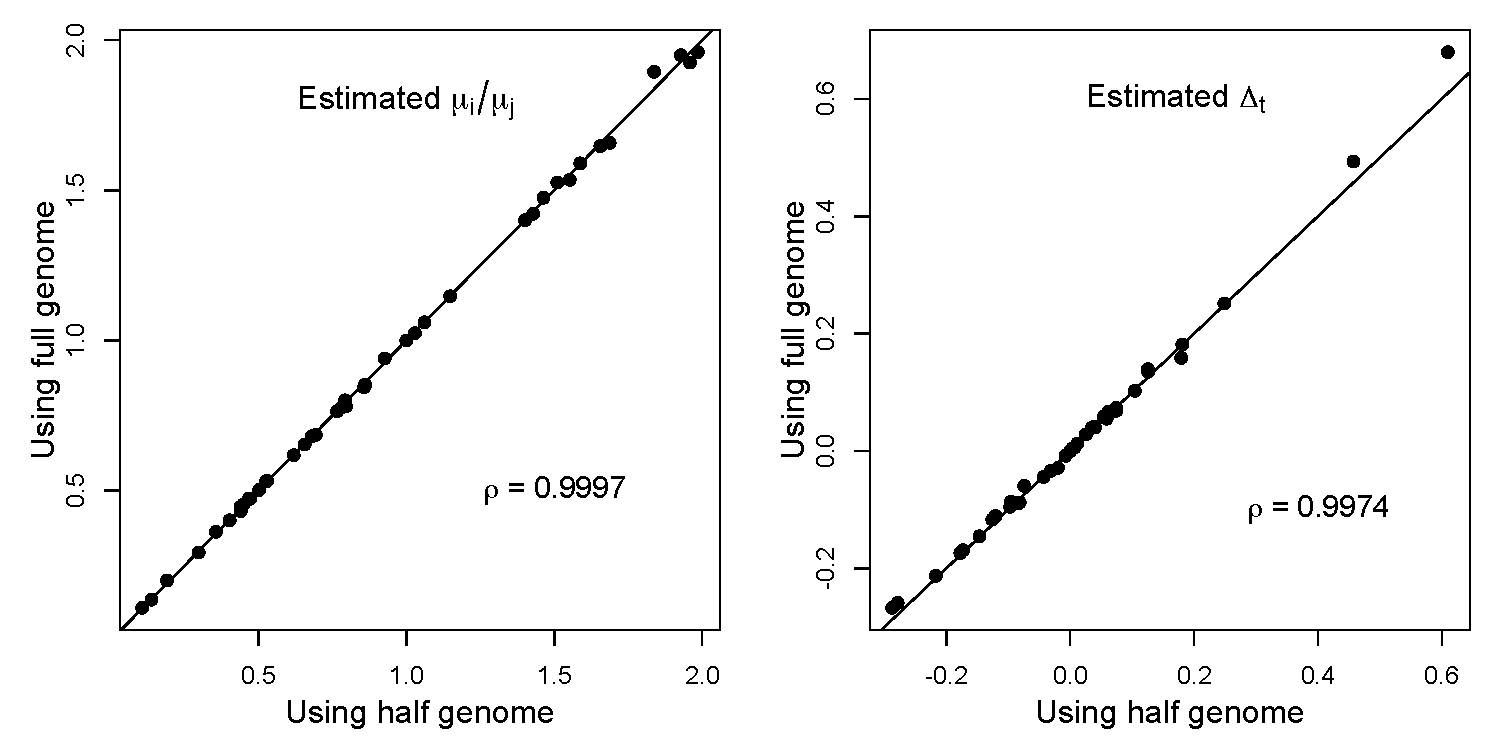
\includegraphics[width=0.9\textwidth]{../Figure/c4Fig_5.pdf}
	\end{center}
                %\includegraphics{./Figures/Shah_fig4.pdf}
	\caption{Correlation between estimates of $\Delta t$s and$\mu_i/\mu_j$ using a random subset of 2337 genes (half the genome) and using the entire genome.}
	We find a strong correlation ($\rho>0.99$, $p$-value $<10^{-15}$) for both $\Delta t$ and $\mu_i/\mu_j$.
	\label{fig:c4_5}
\end{figure}


We then used the parameters estimated using the first set of genes to predict gene-specific  codon counts in the second set of genes.
The correlation coefficient between observed and predicted codon counts at the level of individual genes was 0.96 (Figs. \ref{fig:c4_6} and \ref{fig:c4_7}).

\begin{figure}[H]
        \begin{center}
                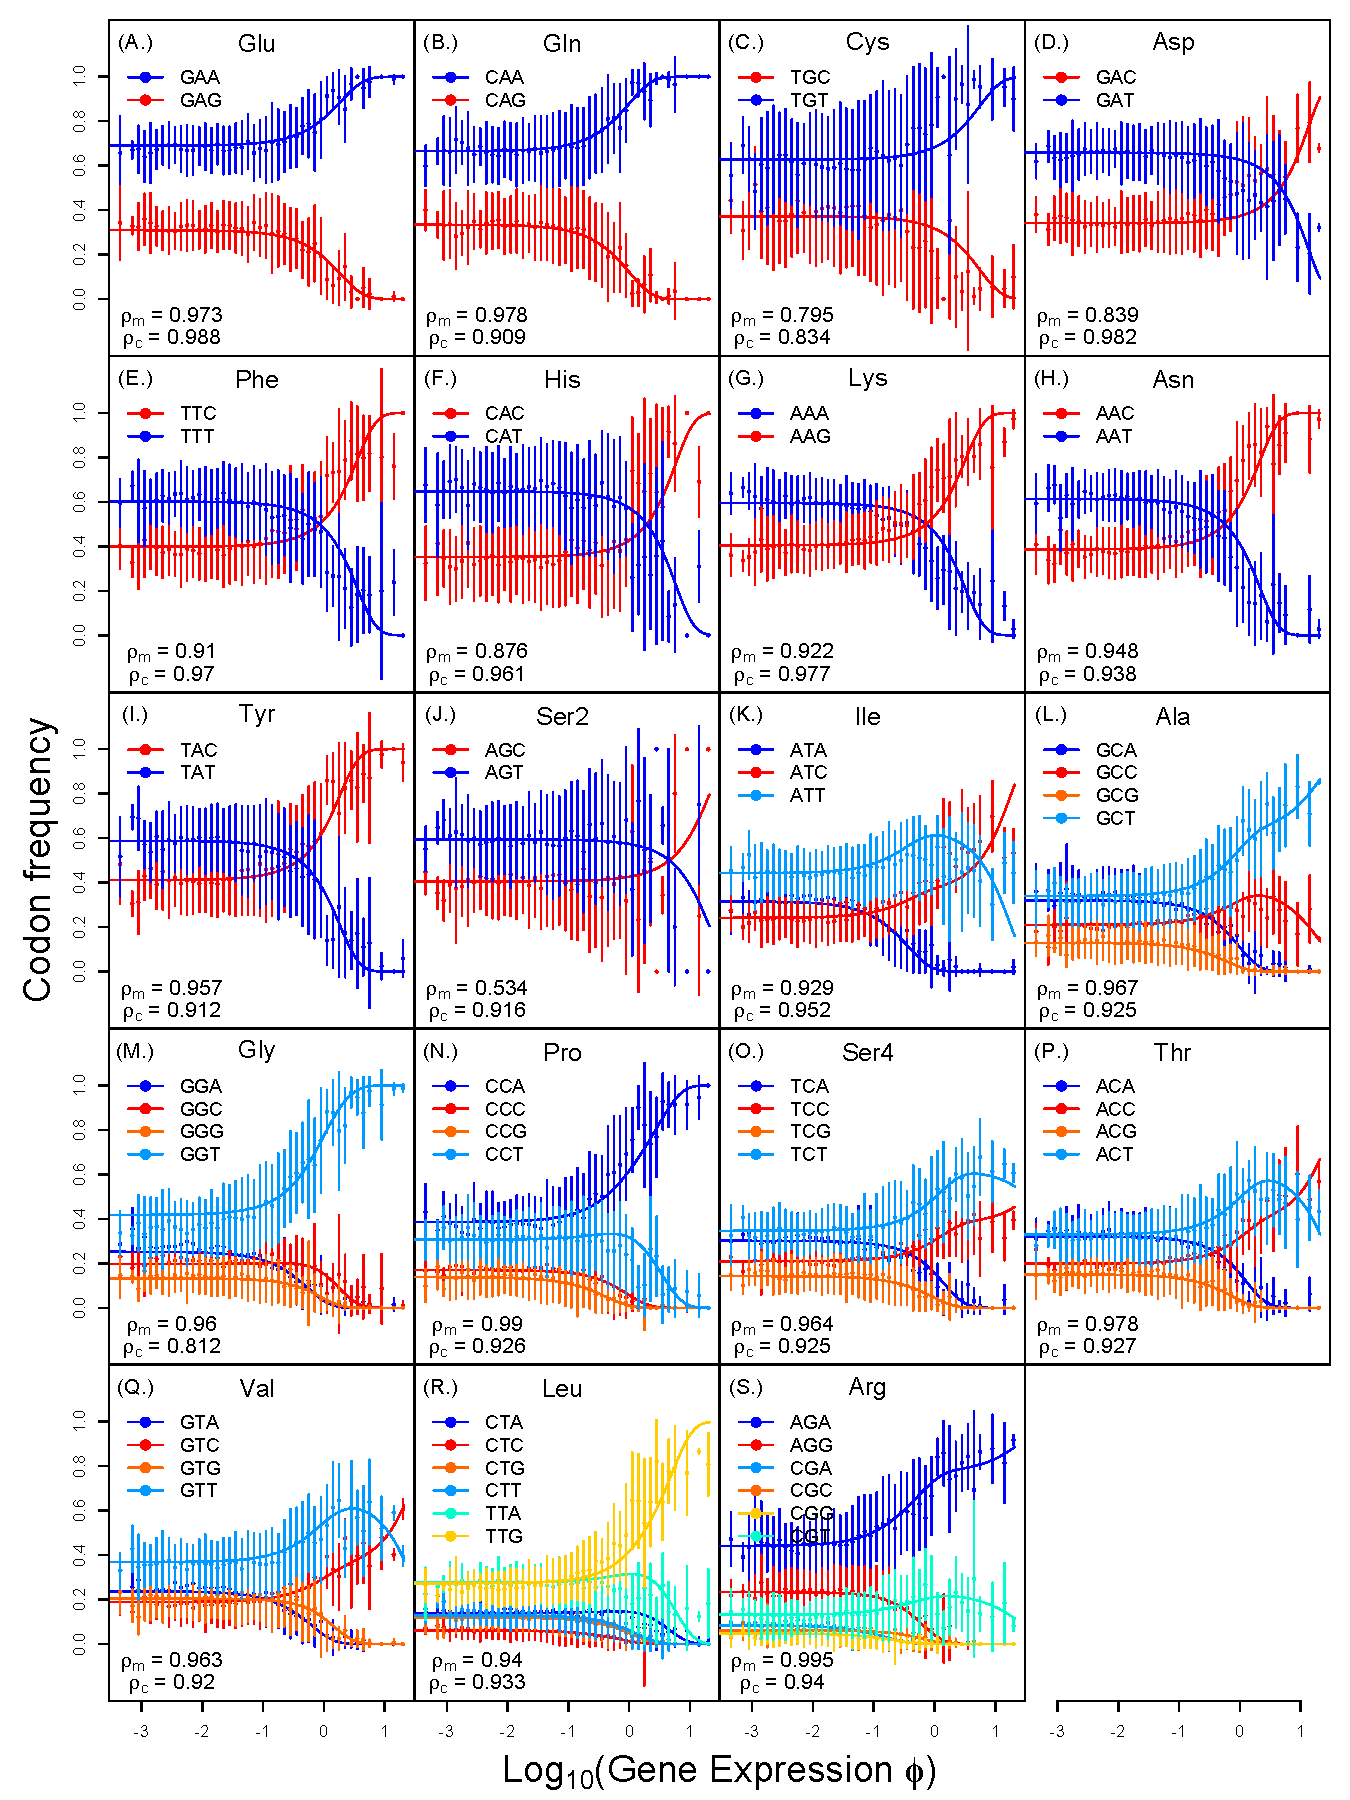
\includegraphics[width=0.75\textwidth]{../Figure/c4Fig_6.pdf}
	\end{center}
	\caption{Observed and predicted changes in codon frequencies with gene expression for the second half of the genome using parameters $\Delta t$ and $\mu_i/\mu_j$ estimated using the first half.}
	Each panel corresponds to a specific amino acid where codons ending in A/T are is shown in shades of blue while codons ending in G/C in shades of red.
	Solid dots and vertical bars represent mean $\pm 1$ SD of observed codon frequencies within genes with protein production rates defined by the bin. 
	The expected codon frequencies under our model are represented by solid lines.
	$\rho_M$ represents the correlation between the mean of observed codon frequencies in a bin and predicted codon frequencies at mean $\phi$ value. 
	$\rho_c$ represent the correlation between observed codon counts and predicted codon counts of all genes at their specific $\phi$ value.
	\label{fig:c4_6}
\end{figure}

\begin{figure}[H]
        \begin{center}
                %\includegraphics[width=0.9\textwidth]{./Figures/tmp3.pdf}
              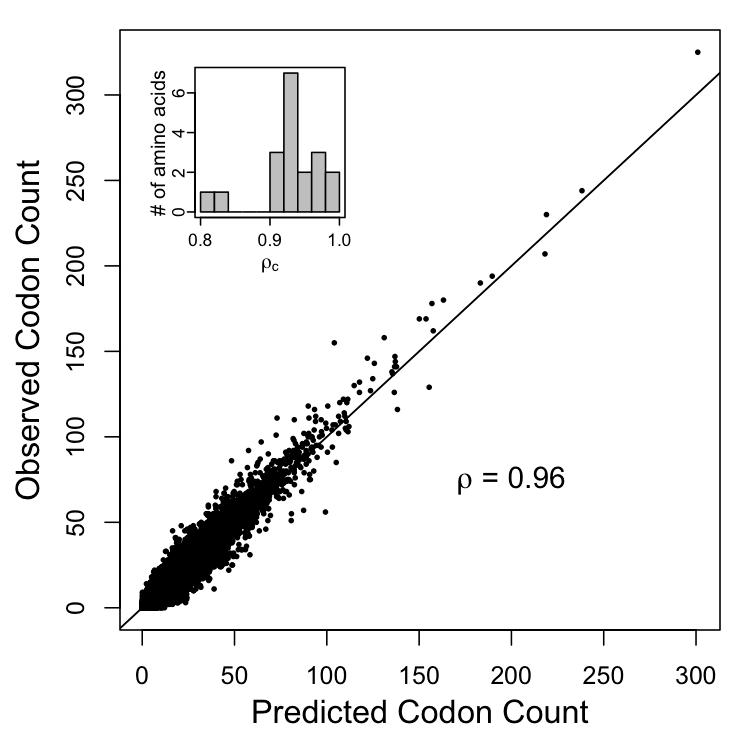
\includegraphics{../Figure/c4Fig_7.pdf}
	\end{center}
	\caption{Correlation between observed codon counts and predicted codon counts of individual genes in second half of the genome using parameters $\Delta t$ and $\mu_i/\mu_j$ estimated using the first half.}
	We find a very high correlation ($\rho=0.96$, $p$-value $<10^{-15}$) between our model predictions and observed counts.
	Inset shows the distribution of correlation coefficients at the level of individual amino acids, indicating that our high correlation is not biased by specific amino acids and that we have a high correlation across all amino acids.
	\label{fig:c4_7}
\end{figure}


Since for most organisms we do not have ribosome occupancy datasets to estimate protein production rates, we estimated $\Delta t_{ij}$ and $\mu_i/\mu_j$ using mRNA abundances \citep{BeyerEtAl04,Gilchrist07} as proxies for protein production rates $\phi$.
We found a very high correlation between parameters estimated using mRNA abundances and protein production rates ($\rho>0.97$, Figs. \ref{fig:c4_8} and \ref{fig:c4_9}). 
Because our model is based on mechanistic principles of protein translation, these parameters can be directly related to specific biological processes underlying protein translation. 
Our work demonstrates that, in principle, these parameters can be estimated directly from genomic and expression datasets, as shown above.
Estimation of these parameters can thus be easily extended to any sequenced organisms for which genome scale expression datasets exist.

\begin{figure}[H]
        \begin{center}
                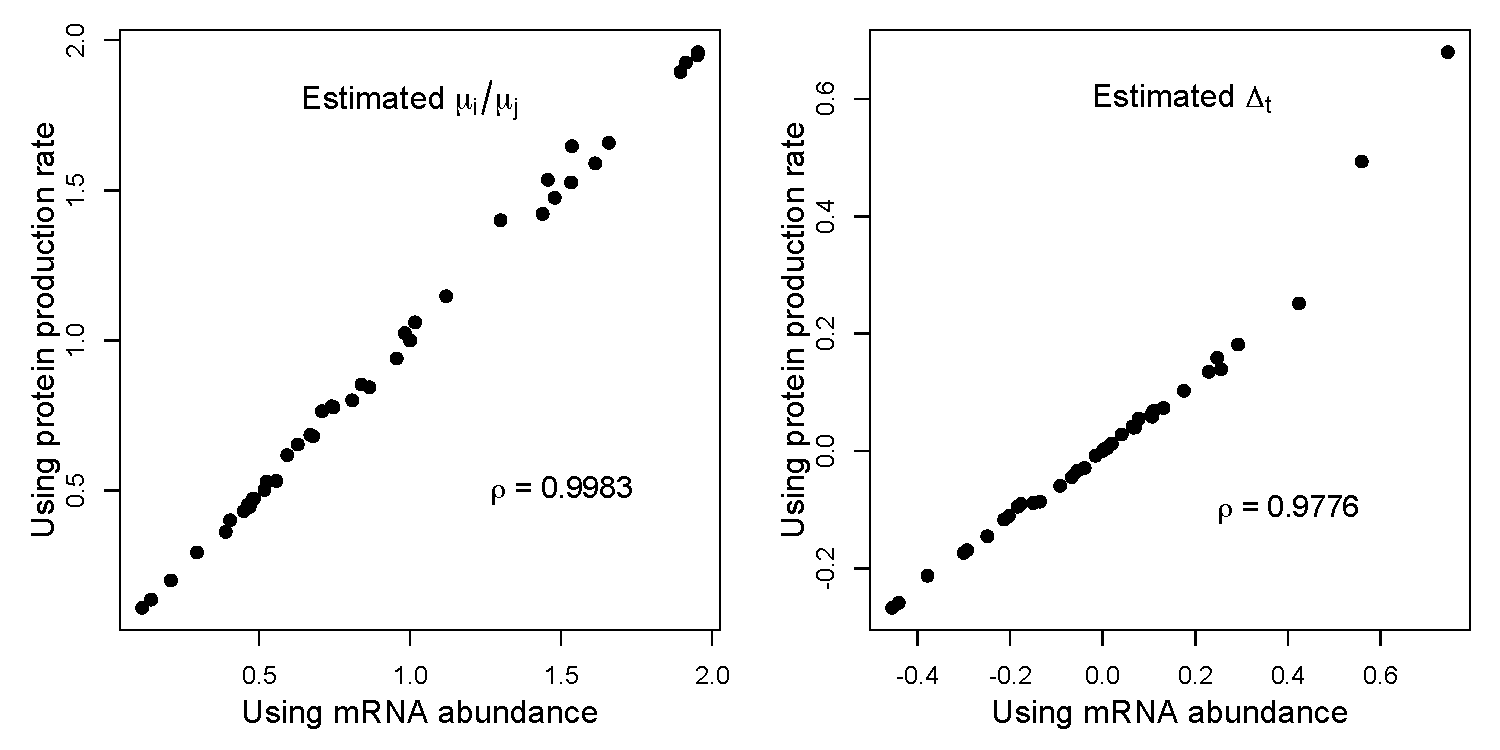
\includegraphics[width=0.9\textwidth]{../Figure/c4Fig_8.pdf}
	\end{center}
                %\includegraphics{./Figures/Shah_fig4.pdf}
	\caption{Correlation between estimates of $\Delta t$s and$\mu_i/\mu_j$ using protein production rates $\phi$ for each gene and using mRNA abundances.}
	We find a strong correlation ($\rho>0.97$, $p$-value $<10^{-15}$) for both $\Delta t$ and $\mu_i/\mu_j$.
	\label{fig:c4_8}
\end{figure}

\begin{figure}[H]
        \begin{center}
                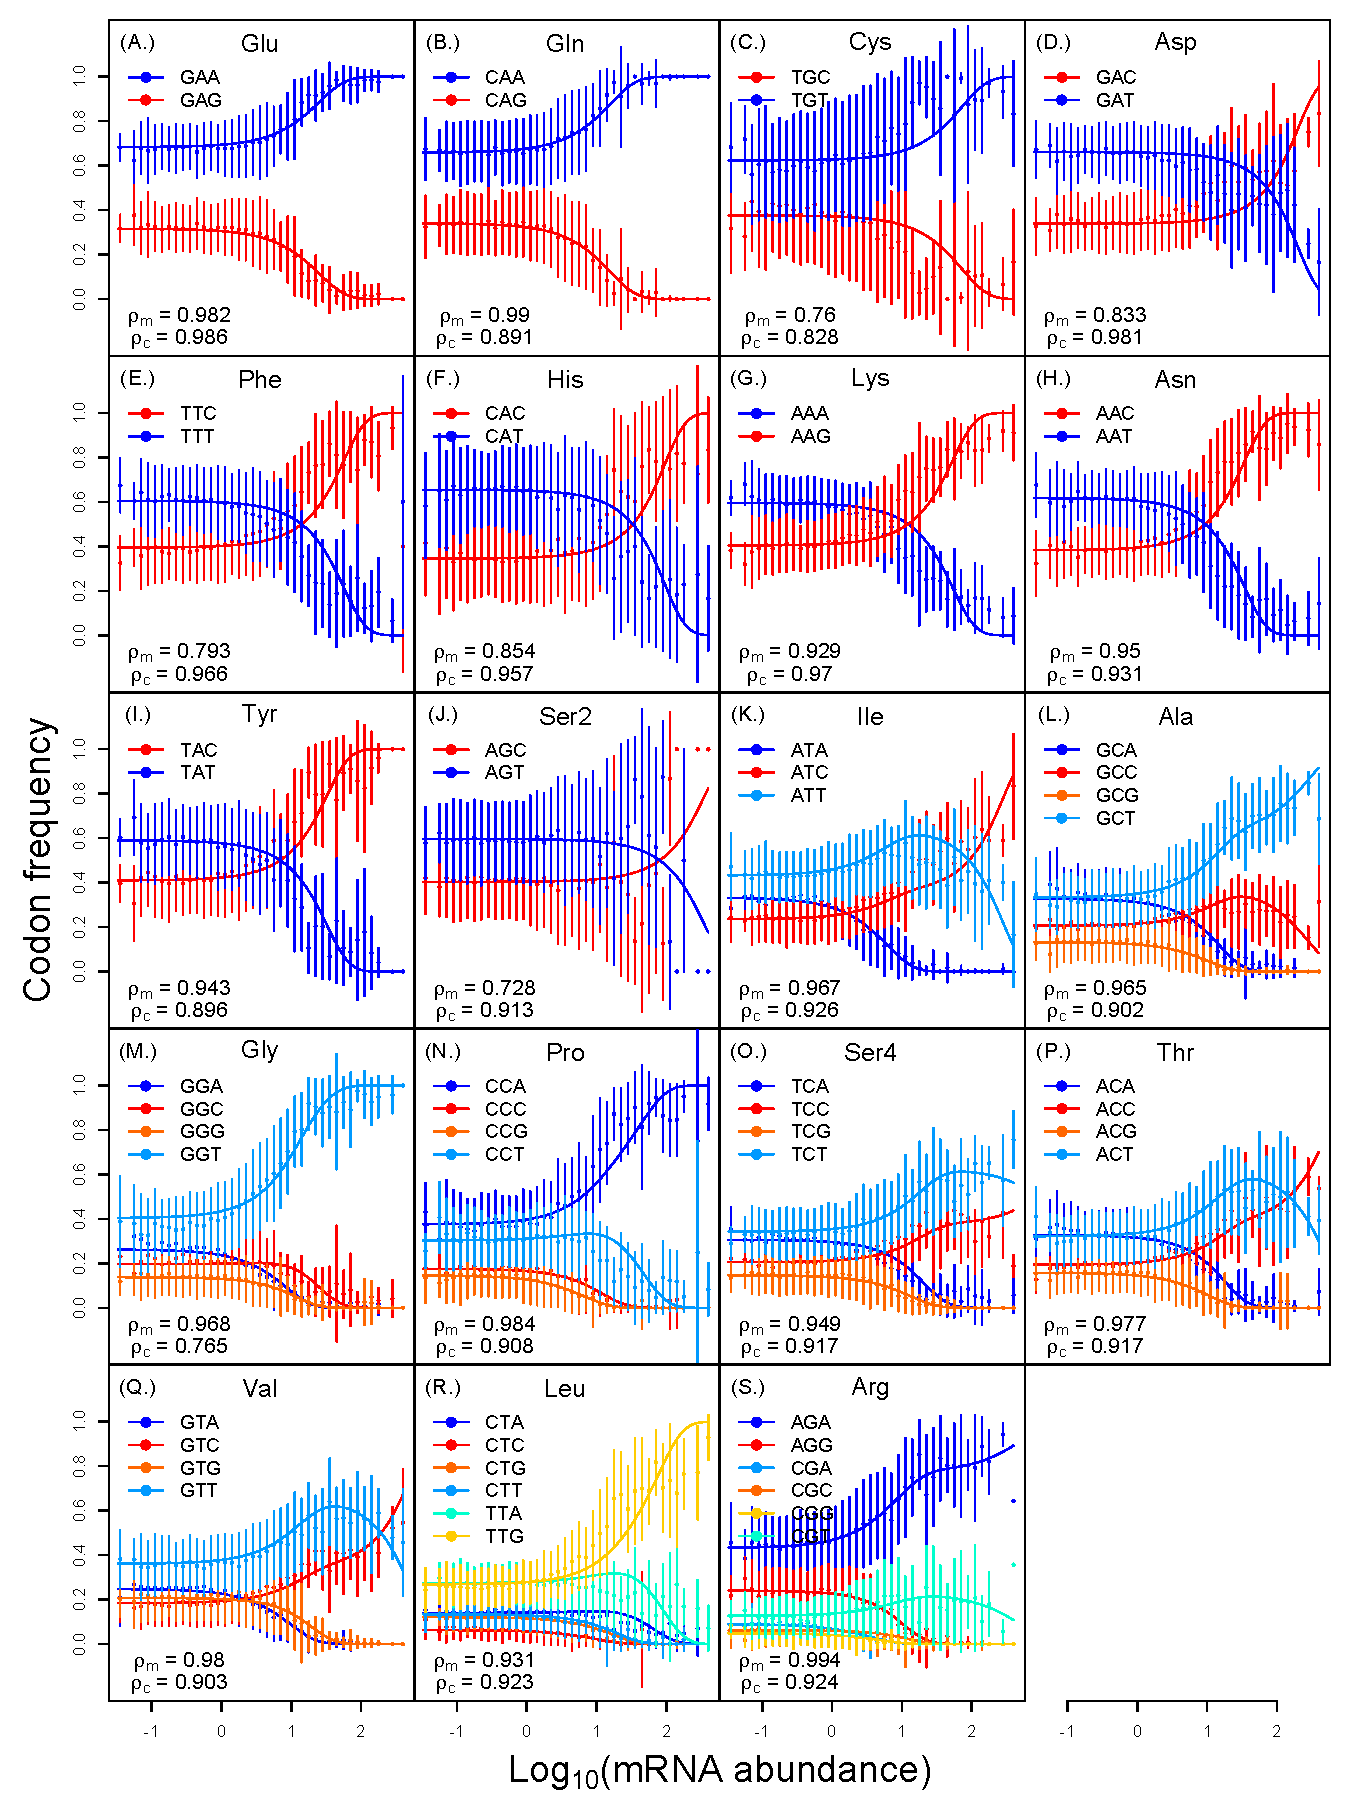
\includegraphics[width=0.75\textwidth]{../Figure/c4Fig_9.pdf}
	\end{center}
	\caption{Observed and predicted changes in codon frequencies with gene expression, specifically mRNA abundances.}
	Each panel corresponds to a specific amino acid where codons ending in A/T are is shown in shades of blue while codons ending in G/C in shades of red.
	Solid dots and vertical bars represent mean $\pm 1$ SD of observed codon frequencies within genes with mRNA abundances defined by the bin. 
	The expected codon frequencies under our model are represented by solid lines.
	$\rho_M$ represents the correlation between the mean of observed codon frequencies in a bin and predicted codon frequencies at mean mRNA abundance of the bin. 
	$\rho_c$ represent the correlation between observed codon counts and predicted codon counts of all genes at their specific $\phi$ value.
	\label{fig:c4_9}
\end{figure}

\section{Discussion}
\subsection{Broader Interpretation of $\Delta t_{ij}$.}
The high correlation between estimates of $\Delta t_{ij}$ from independent sources of genomic information (Fig. \ref{fig:c4_4}), suggests that our interpretation of the term $\Delta t_{ij}$ is consistent with selection for translation efficiency as a major force in shaping patterns of codon usage.
However, from a purely mathematical standpoint, the parameter $\Delta t_{ij}$ is akin to the additive fitness component used in \citep{SellaAndHirsh05}, scaled by $\phi$.
Thus its value can broadly be interpreted as an expression level dependent selective coefficient associated with the specific codon pair.
In future, this broader interpretation should allow us to compare our genome-based estimates of $\Delta t_{ij}$ with values expected under alternate hypotheses of the factors responsible for shaping codon usage patterns.
For example, in the case of Cys, an interpretation of $\Delta t_{ij}$ is difficult to justify based on a naive model of estimating elongation times from tRNA abundances. 
In \emph{S. cerevisiae}, Cys is coded by a single tRNA where the non-canonical codon TGT is recognized by wobble and assumed to be elongated at a slower rate than its synonym TGC \citep{GromadskiAndRodnina04, ShahAndGilchrist10b}.
Thus, our estimates of $t_\text{TGT}-t_\text{TGC}<0$ cannot be explained on the basis of elongation times alone as the sign of $\Delta t_{TGT,TGC}$ is opposite to that expected based on tRNA abundances and wobble. 
A variety of factors could potentially explain this discrepancy.
Firstly, due to its unique ability to form disulphide linkages, Cys might be under a stronger selection to minimize missense errors than other amino acids.
The fact that a codon with a slower elongation rate might be better at minimizing missense errors has also been predicted in a large number of other microorganisms \citep{ShahAndGilchrist10b}.
Secondly, as noted by \citep{BennetzenAndHall82}, codons with side-by-side GC nucleotides may be selected against due to the high binding energies between codon-anticodon pairs.
Despite the fact that $\Delta t_{ij}$ can potentially be interpreted many ways, the high correlation between our predicted $\Delta t_{ij}$ and estimates of $\Delta t_{ij}$ based simply on tRNA gene copy numbers and wobble parameters (Fig. \ref{fig:c4_4}) indicates a mechanistic link between our estimates of $\Delta t$ and differences in elongation times of codons.

In summary, our work shows that genome scale patterns of codon usage can be largely explained by the effects of genetic drift, mutational biases, and natural selection for efficient usage of ribosome, i.e. translational efficiency.
Although a variety of indices have been proposed to estimate the degree of adaptation of a gene based on its codon usage bias, ours method makes predictions in the opposite direction as well, i.e., predicting codon counts of a gene given its expression level.
Our model of translation efficiency also allows us to estimate codon-specific elongation times (selection coefficients) as well as relative mutation rates.
In addition, we make quantitative predictions on how individual codon frequencies should change with gene expression in yeast.
Although, selection for translational efficiency appears to be sufficient to explain most of the genome-scale patterns of codon usage this does not preclude the effects of other selective forces on the evolution of CUB.
For instance, selection for translation accuracy (minimizing translation missense errors) has long been argued to be a dominant force in driving the evolution of CUB \citep{Akashi94,DrummondEtAl05,DrummondAndWilke08}.
However, current data suggests that only $\sim10-50\%$ of missense errors disrupt protein function \citep{MarkiewiczEtAl94,GuoEtAl04}, and therefore cannot explain the high frequencies $\sim$100\%  of mutationally disfavored codons in Phe, Asn, and Tyr amino acids (Fig. \ref{fig:c4_2}).
Moreover, the assumptions underlying Akashi�s test \citep{Akashi94} used to support the translation accuracy hypothesis are not always justified \citep{ShahAndGilchrist10b}. 
Nevertheless, selection for translation accuracy can explain codon usage at functionally and/or structurally critical sites of a protein \citep{DrummondAndWilke08}. 
Because codons that minimize missense errors may not necessarily be the ones that minimize elongation times \citep{ShahAndGilchrist10b}, our model is likely insufficient to explain the codon usage at these sites. 
Similarly, adaptation against nonsense errors has been documented in \emph{S. cerevisiae} \citep{GilchristAndWagner06,GilchristEtAl09} and other organisms \citep{QinEtAl04}.
In addition, factors indirectly related to protein translation, such as  mRNA secondary structures at the $5'$ region of a gene, have been shown to be under selection for translation initiation and hence can effect the frequency of codon usage at these sites \citep{KudlaEtAl09,TullerEtAl10b}.


Clearly, although a number of selective mechanisms have been proposed to explain and likely contribute to specific patterns of codon usage, the combined effects of these forces in shaping genomic patterns of codon usage are not well understood \citep{DrummondAndWilke09,PlotkinAndKudla11}.
In order to decipher the relative importance of these forces on the evolution of CUB, mechanistic models that explicitly take into account tRNA competition and intra-ribosomal dynamics \citep{ShahAndGilchrist10b} as well as effects of amino acid substitutions on protein structure and function \citep{GuoEtAl04} need to be developed.
%include these other potential selective forces must be developed.
Our model demonstrates the strength of such an approach and provides a natural framework for expansion to include other selective forces as well.
More generally, this approach will allow us to quantitatively estimate parameters underlying fundamental biological processes such as protein translation and improve our understanding of how evolutionary forces shape genomic patterns and processes.

%% == end of paper:

%% Optional Materials and Methods Section
%% The Materials and Methods section header will be added automatically.

%% Enter any subheads and the Materials and Methods text below.
\section{Methods}\label{sec:meth}
\subsection{Estimation of $\Delta t_{ij}$ and $\mu_i/\mu_j$ from observed data}
%In order to estimate codon-pair specific differences in elongation times $\Delta t_{ij}$ and relative mutation rates $\mu_i/\mu_j$, we obtained gene expression data, specifically protein production rates $\phi$ of genes in \emph{S. cerevisiae} estimated in \citep{Gilchrist07}.
%These estimates of protein production rates are based on mRNA abundance data from \citep{BeyerEtAl04} and ribosome occupancy data from  \citep{AravaEtAl03,MacKayEtAl04}.
In the case of an amino acid with $k$ codons, the change in codon frequencies across the entire range of gene expression can be determined by $2(k-1)$ parameters for codon-specific mutation rates and elongation times. 
For instance, in the case of amino acids with two codons, the frequency of any one codon depends only on the \emph{difference} in the elongation times of the two codons and the ratio of their mutation rates.
\begin{align}
\mathbb{E}[x_1|\phi]&=\frac{n\mu_1e^{-N_e q C\phi t_1}}{\mu_1e^{-N_e q C\phi t_1} + \mu_2e^{-N_e q C\phi t_2}}\nonumber\\
&=\frac{1}{1 +  \frac{\mu_2}{\mu_1}e^{-N_e q C\phi (t_2-t_1)}}
\end{align}

%\section{Estimation of relative mutation rates}
%\section{Estimation of relative mutation rates and differences in elongation times}
Codon usage in genes with low expression $\phi$ is thought to be determined primarily by mutation biases, i.e., $N_e q C\phi\approx0$.
Since absolute mutation rates to each codon cannot be estimated directly as it is only their ratios that affect codon usage, we estimated $\mu_i/\mu_j$ by setting the mutation rate of an arbitrarily chosen codon to 1.
Codon counts in low expression genes can then be assumed to follow a multinomial distribution with parameters determined by their mutation rates.
Thus, in the case of an amino acid with two codons whose codon counts are $x_1$ and $x_2$, the maximum likelihood estimate of relative mutation rate is approximately,
\begin{align}
\frac{\mu_2}{\mu_1}\approx\frac{x_2}{x_1}
\end{align}

Similarly, elongation times of codons affect codon usage only as their {differences} ($t_1-t_2$).
Thus, during parameter estimation of elongation times, we set the elongation time of an arbitrarily chosen codon within each amino acid to 1 and estimated the differences in elongation times of other codons with respect to that codon.
%We further binned genes based on their protein production rates $\phi$, into 50 categories.
%The mean frequencies of codons across genes within each bin we used for parameter estimation.
We used the NEWUOA optimization algorithm \citep{Powell06} employed in R to estimate $\Delta t_{ij}$ and $\mu_i/\mu_j$ for an amino acid with $k$ codons and $qC$ by maximizing the following likelihood function (see Section \ref{text:c4_1} for additional details).
\begin{align}
\text{Lik}(\vec{t},\vec{\mu}|\phi,\vec{x})=P(\vec{x}|\phi)=\prod_{i=1}^k\left(\frac{\mu_ie^{-N_e q C\phi t_i}}{\sum_{j=1}^{k}\mu_je^{-N_e q C\phi t_j}}\right)^{x_i}
\end{align}
In addition, we estimated the maximum likelihood value of $\widehat{qC}=9.12\times10^{-7}$ .

\subsection{Estimation of $\Delta t_{ij}$ from tRNA gene copy numbers}
In order to compare our estimates of $\Delta t_{ij}$ with an independent source of genomic information, we estimated $\Delta t_{ij}$ using tRNA gene copy numbers and wobble effects.
Following  \citep{DongEtAl96,KanayaEtAl99}, we use tRNA gene copy numbers in yeast obtained from GtRNAdb \citep{ChanAndLowe09} as proxies for tRNA abundances.
We assume that the expected waiting time at a codon $t_i$ is inversely proportional to its cognate tRNA abundances based on an exponential waiting process.
\begin{align}
\text{[tRNA$_i$]} &\propto\text{Gene copy number of tRNA$_i$}\\
%t_i &= &\frac{a}{\sum_{j\in S_{cog}}\text{[tRNA$_j$]} \times w_{j,i}}
t_i &= \frac{a}{\text{[tRNA$_i$]} \times wob}
\end{align}
where $wob$ is the wobble penalty due to codon-anticodon mismatch and $a$ is a scaling constant.
When a codon is recognized by its canonical tRNA, we set $wob=1$.
Based on \citep{CurranAndYarus89,LimAndCurran01}, we assume that a purine-purine or pyrimidine-pyrimidine wobble penalty to be 39\% and purine-pyrimidine wobble penalty to be 36\%.
We set the scaling constant $a$ such that the harmonic mean of elongation rates of all codons is 10 aa/sec \citep{GilchristAndWagner06,Gilchrist07}.
However, note that changing the scaling constant would have no effect on the correlation between our model based and gene copy number based estimates of $\Delta t_{ij}$.

%% Optional Appendix or Appendices
%% \appendix Appendix text...
%% or, for appendix with title, use square brackets:
%% \appendix[Appendix Title]

\section{Acknowledgements}
We thank J. Plotkin, B. O'Meara, F. Ubeda de Torres, I. Juric %and two anonymous reviewers 
for their comments on the manuscript.
Support for this project was provided by Department of Ecology and Evolutionary Biology
at University of Tennessee, Knoxville, the National Institute for Mathematical and Biological
Synthesis (NIMBioS), and the TN Science Alliance.  
P.S. was additionally funded by a NIMBioS  Graduate Research Assistantship.
%M.A.G. would like to thank B. Burstein and S. Gardial for their indirect support of this work.

\clearpage
\pagebreak

\section{Supporting Information}
\subsection{Analytical solutions of the model}{\label{text:c4_1}}
\subsubsection{One amino acid with two codons}

Consider a gene sequence of length $n$ composed of a single two-codon amino acid, whose average elongation times are $t_1$ and $t_2$. 
Let $x_1$ and $x_2=n-x_1$ be the respective codon counts.
The expected cost of ribosome usage during protein production is then given as
\begin{align}
\eta(\vec{x})&=C\sum_{i=1}^{2}x_it_i\\
&=C(x_1 t_1 + x_2 t_2)
\end{align}
where $C$ is the cost of ribosome usage in ATP/sec. We assume an exponential fitness function $w$ described as
\begin{align}
w(\vec{x}|\phi)&=e^{-q\phi\eta(\vec{x})}=e^{-q\phi C(x_1 t_1 + x_2 t_2)}
\end{align}
where $\phi$ is the protein production rate, a measure of gene expression and $q$ is the scaling constant determining the relationship between cost of ATP usage to organismal fitness $w$.

Following \citep{Kimura64, Gavrilets04B, BergEtAl04,  SellaAndHirsh05}, the probability of observing an allele across the entire genotype space at equilibrium is given by 
\begin{align}
P(\vec{x}|\phi)&=\frac{w(\vec{x}|\phi)^{N_e}}{\sum_{y\in S_c}w(\vec{y}|\phi)^{N_e}}
\end{align}
where $N_e$ is the effective population size and $S_c$ is the entire synonymous codon genotype space, which has $2^n$ alleles in this simple case.
Since the cost of protein production is independent of codon order within a gene, multiple synonymous alleles could give rise to the same cost $\eta$.
In the 2 codon case, the number of alleles with the same cost is represented by a binomial coefficient and for amino acids with more than two codons, the combinations will be represented by a multinomial coefficient.
\begin{align}
P(\vec{x}|\phi)&=\frac{\binom{n}{x_1}e^{-N_e q \phi C (x_1 t_1 + x_2 t_2)}}{\sum_{y_1=0}^{n}\binom{n}{y_1}e^{-N_e q \phi C(y_1 t_1 + y_2 t_2)}}
\end{align}
Let $\mu_1$ and $\mu_2$ represent the rate of mutations \emph{to} the two codons as described by \citep{SellaAndHirsh05}.
For instance, $\mu_1=\mu_{21}$ indicates the rate at which codon 2 is mutated to codon 1.

Taking mutational biases into account, the probability of observing a given allele is given as
\begin{align}
P(\vec{x}|\phi)&\propto w(\vec{x}|\phi)^{N_e}\prod_{i=1}^2\mu_i^{x_i}\\
P(\vec{x}|\phi)&=\frac{\binom{n}{x_1}e^{-N_e q C \phi (x_1 t_1 + x_2 t_2)}\prod_{i=1}^2\mu_i^{x_i}}{\sum_{y_1=0}^{n}\binom{n}{y_1}e^{-N_e q C \phi (y_1 t_1 + y_2 t_2)}\prod_{i=1}^2\mu_i^{y_i}}
%&=\frac{\binom{n}{x_1}e^{N_e (x_1( \mu_1 - q C\phi t_1)+  x_2(\mu_2 - q C\phi t_2))}}{\sum_{y_1=0}^{n}\binom{n}{y_1}e^{N_e(y_1( \mu_1 - q C\phi t_1)+  y_2(\mu_2 - q C\phi t_2))}}
\end{align}
where $\vec{x}=\{x_1,x_2\}$.

Given the protein production rate $\phi$ (gene expression) of a gene and the elongation times $t$ of codons, the expected count of each codon is given as
\begin{align}
\mathbb{E}[x_1|\phi]&=\sum_{x_1=0}^n x_1P(\vec{x}|\phi)\\
&=\sum_{x_1=0}^n x_1\frac{\binom{n}{x_1}e^{-N_e q C \phi (x_1 t_1 + x_2 t_2)}\prod_{i=1}^2\mu_i^{x_i}}{\sum_{y_1=0}^{n}\binom{n}{y_1}e^{-N_e q C \phi (y_1 t_1 + y_2 t_2) }\prod_{i=1}^2\mu_i^{y_i}}\\
&=\frac{n\mu_1e^{-N_e q C\phi t_1}}{\mu_1e^{-N_e q C\phi t_1} + \mu_2e^{-N_e q C\phi t_2}}
\end{align}
and by symmetry
\begin{align}
\mathbb{E}[x_2|\phi]&=\frac{n\mu_2e^{-N_e q C\phi t_1}}{\mu_1e^{-N_e q C\phi t_1} + \mu_2e^{-N_e q C\phi t_2}}\\
&=n-\mathbb{E}[x_1|\phi]
\end{align}

\subsubsection{One amino acid with $k$ codons}
Using the methods described above it can be showed that for any amino acid with $k$ codons, the expected count of the $i^{th}$ codon is given as
\begin{align}
\mathbb{E}[x_i|\phi]&=\frac{n\mu_ie^{-N_e q C\phi t_i}}{\sum_{j=1}^{k}\mu_je^{-N_e q C\phi t_j}}
\end{align}
Thus, the expected frequencies of each codon $f_i=x_i/n$ is given as
\begin{align}
\mathbb{E}[f_i|\phi]&=\frac{\mu_ie^{-N_e q C\phi t_i}}{\sum_{j=1}^{k}\mu_je^{-N_e q C\phi t_j}}
\end{align}

Variance around the expected value $\mathbb{E}x_i|\phi$ can also be calculated as
\begin{align}
\text{Var}[x_i|\phi]&=\sum_{x_i=0}^n (x_i - \mathbb{E}x_i|\phi)^2 P(\{x_1,x_2,\cdots,x_k\})\\
&=\frac{n\left(\prod_{j=1}^{k}\mu_j\right)e^{N_e q C \phi \sum_{j=1}^{k} t_j}}{\left(\sum_{j=1}^{k}\mu_je^{N_e q C \phi t_j}\right)^2}
\end{align}

\subsubsection{Multiple amino acids with varying number of codons}
In the case of real genes, which are comprised of multiple amino acids each with a varying number of codons, the expected counts and frequencies of codons can be estimated from the marginal distributions of each amino acid.
For instance, consider the simple case of two amino acids with two codons each.
The ribosomal overhead cost of protein production is given as
\begin{align}
\eta(\vec{x})&=C(x_{11} t_{11} + x_{12} t_{12} + x_{21} t_{21} + x_{22} t_{22})
\end{align}
where $x_{ij}$ is the number of codons of type $j$ of amino acid $i$ in the gene. Let $n_1=x_{11}+x_{12}$ and $n_2=x_{21}+x_{22}$ be the counts of the two amino acids in the gene. 
As earlier, the probability of observing an allele can be written as
\begin{align}
P(\vec{x}|\phi)=&\frac{\binom{n_1}{x_{11}}\binom{n_2}{x_{21}}\prod_{j=1}^{2}\mu_{1j}^{x_{1j}}\prod_{j=1}^{2}\mu_{2j}^{x_{2j}}e^{-N_e (x_{11} q C\phi t_{11}+  x_{12} q C\phi t_{12} +  x_{21} q C\phi t_{21}+  x_{22} q C\phi t_{22})}}{\sum_{y_{11}=0}^{n_1}\sum_{y_{21}=0}^{n_2}\binom{n_1}{y_{11}}\binom{n_2}{y_{21}}\prod_{j=1}^{2}\mu_{1j}^{y_{1j}}\prod_{j=1}^{2}\mu_{2j}^{y_{2j}}e^{-N_e (y_{11} q C\phi t_{11}+  y_{12} q C\phi t_{12} +  y_{21} q C\phi t_{21}+  y_{22} q C\phi t_{22})}}\\
%&=\frac{\binom{n_1}{x_{11}}e^{N_e (x_{11}( \mu_{11} - q C\phi t_{11})+  x_{12}(\mu_{12} - q C\phi t_{12}))} \times \binom{n_2}{x_{21}} e^{N_e (x_{21}(\mu_{21} - q C\phi t_{21})+  x_{22}(\mu_{22} - q C\phi t_{22}))}}{\sum_{y_{11}=0}^{n_1}\binom{n_1}{y_{11}}e^{N_e (y_{11}( \mu_{11} - q C\phi t_{11})+  y_{12}(\mu_{12} - q C\phi t_{12}))} \times \sum_{y_{21}=0}^{n_2}\binom{n_2}{y_{21}} e^{N_e (y_{21}(\mu_{21} - q C\phi t_{21})+  y_{22}(\mu_{22} - q C\phi t_{22}))}}\\
=&\frac{
\binom{n_1}{x_{11}}\prod_{j=1}^{2}\mu_{1j}^{x_{1j}}e^{-N_e (x_{11} q C\phi t_{11}+  x_{12} q C\phi t_{12})}
}
{
\sum_{y_{11}=0}^{n_1}\binom{n_1}{y_{11}}\prod_{j=1}^{2}\mu_{1j}^{x_{1j}}e^{-N_e (x_{11} q C\phi t_{11}+  x_{12} q C\phi t_{12})}
} \times\nonumber\\
&\frac{
\binom{n_2}{x_{21}}\prod_{j=1}^{2}\mu_{2j}^{x_{2j}}e^{-N_e (x_{21} q C\phi t_{21}+  x_{22} q C\phi t_{22})}
}
{
\sum_{y_{21}=0}^{n_2}\binom{n_2}{y_{21}} \prod_{j=1}^{2}\mu_{2j}^{x_{2j}}e^{-N_e (x_{21} q C\phi t_{21}+  x_{22} q C\phi t_{22})}
}\\
P(\{\vec{x}_1,\vec{x}_2\})&=P(\vec{x}_1|aa_1)P(\vec{x}_2|aa_2)
\end{align}
The marginal distribution of genotype space of a singe amino acid is given as
\begin{align}
\sum_{x_{21}=0}^{n_2}P(\vec{x}_2|aa_2)&=1\\
P(\vec{x}_1|aa_1)&=\sum_{x_{21}=0}^{n_2}P(\{\vec{x}_1,\vec{x}_2\})
\end{align}

Thus, the expected number of codons of a specific amino acid based on the marginal distribution of that amino acid can be calculated as
\begin{align}
\mathbb{E}[x_{11}|\phi]&=\sum_{x_{11}=0}^{n_1} x_{11}\sum_{x_{21}=0}^{n_2}P(\{\vec{x}_1,\vec{x}_2\})\\
&=\sum_{x_{11}=0}^{n_1} x_{11}P(\vec{x}_1|aa_1)\sum_{x_{21}=0}^{n_2}P(\vec{x}_2|aa_2)\\
&=\sum_{x_{11}=0}^{n_1} x_{11}P(\vec{x}_1|aa_1)\\
&=\frac{n_1\mu_{11}e^{-N_e q C\phi t_{11}}}{\mu_{11}e^{-N_e q C\phi t_{11}} + \mu_{12}e^{-N_e q C\phi t_{12}}}
\end{align}
The above Eqn. (27) is equivalent to Eqn. (11) which considers a gene sequence with only one amino acid and two codons.

\subsection{An argument against model over-parametrization}{\label{text:c4_2}}
Although, it may seem that the excellent fit between the observed and predicted values may be due to over-fitting the data with a large numbers of parameters, this is not the case.
For instance, in the case of an amino acid with $k$ codons, there are $k-1$ independent codon frequencies.
Since the change in codon frequencies with gene expression can be thought of as a non-linear regression, each codon should have a slope and an intercept.
Thus there are $2(k-1)$ independent parameters for an amino acid with $k$ codons.
The relative mutation rates provide the estimates for intercepts, while differences in elongation times provide the estimates for their respective slopes.
The beauty of our approach lies in the fact that our simple model, appropriately parameterized leads to a correlation coefficient of 0.96.


\pagebreak